\documentclass[aspectratio=169]{beamer}
\usepackage{color,amsmath}
\usepackage{subfigure}
\usepackage{booktabs}
\usepackage{framed}
\usepackage{comment}
\usepackage{hyperref}
\usepackage{ulem}

\usepackage{hyperref}
\hypersetup{
    colorlinks=true,
    linkcolor=blue,
    filecolor=magenta,      
    urlcolor=cyan,
}


%\usepackage{tikz}
%\beamertemplatenavigationsymbolsempty
%\usetikzlibrary{arrows,shapes.arrows,positioning,shapes}
%\newcommand\red[1]{{\color{red}#1}}
%\newcommand\bred[1]{{\color{red}\textbf{#1}}}
%\newcommand\blue[1]{{\color{blue}#1}}
%\newcommand\bblue[1]{{\color{blue}\textbf{#1}}}
%\newcommand\green[1]{{\color{olive}#1}}
%\newcommand\bgreen[1]{{\color{olive}\textbf{#1}}}
%\newcommand\black[1]{{\color{black}#1}}
%\newcommand\white[1]{{\color{white}#1}}
%\newcommand\E{\text{E}}
%\newcommand\V{\text{V}}
%\renewcommand\P{\text{P}}


\title{Day 5: Mass collaboration and machine learning}
\author{Matthew J. Salganik\\Department of Sociology\\Princeton University}
\date[]{
\begin{flushright}

\includegraphics[width=0.1\textwidth]{figures/cc-by.png}
\end{flushright}
}

\begin{document}
%%%%%%%%%%%%%%%%%%%%%%%%%%
\frame{\titlepage}
%%%%%%%%%%%%%%%%%%%%%%%%%%%
\begin{frame}

Happy Juneteenth

\vfill
\url{https://www.pbs.org/wnet/african-americans-many-rivers-to-cross/history/what-is-juneteenth/}

\end{frame}
%%%%%%%%%%%%%%%%%%%%%%%%
\begin{frame}

Today is our final organized lunch tables (you are free to self-organize) \pause
\begin{itemize}
\item Juneteenth \pause
\item Hosting a partner location for SICSS 2021\pause
\item Other topics 
\end{itemize}

\vfill
If you want to learn about hosting a partner location but can't attend, talk to Chris or Matt during office hours in week 2

\end{frame}
%%%%%%%%%%%%%%%%%%%%%%%%
\begin{frame}

Feedback on the feedback \pause
\begin{itemize}
\item People liked groups of 3 \pause
\item Group composition seems to matter \pause
\item Still a few struggles with remote collaboration \pause
\item We heard good things about Zoom remote control \pause
\item Tension between structured and open-ended activities \pause
\item Keep the feedback coming . . . .
\end{itemize}

\end{frame}
%%%%%%%%%%%%%%%%%%%%%%%%%
\begin{frame}

Other logistics questions/comments

\end{frame}
%%%%%%%%%%%%%%%%%%%%%%%%
\begin{frame}

Schedule for today:\\
\url{https://compsocialscience.github.io/summer-institute/2020/duke/schedule}

\end{frame}
%%%%%%%%%%%%%%%%%%%%%%%%%
\title{Participating in the Fragile Families Challenge Activity}
\author{{\small Matthew Salganik, Ian Lundberg, Alex Kindel, Sara McLanahan,\\and people from around the world}}
\date[]{
\begin{flushleft}{\tiny Funding for FFCWS provided by NICHD (R01HD36916, R01HD39135, R01HD40421) and a consortium of private foundations, including the Robert Wood Johnson Foundation. Funding for FFC provided by the Russell Sage Foundation, NSF, \& the Overdeck Fund. FFC Board of Advisors: Jeanne Brooks-Gunn, Kathryn Edin, Barbara Engelhardt, Irwin Garfinkel, Moritz Hardt, Dean Knox, Nicholas Lemann, Karen Levy, Sara McLanahan, Arvind Narayanan, Timothy Nelson, Matthew Salganik, Brandon Stewart \& Duncan Watts.}
\end{flushleft}
\begin{flushright}

\includegraphics[width=0.1\textwidth]{figures/cc-by.png}
\end{flushright}
}

%%%%%%%%%%%%%%%%%%%%%%%%%
\frame{\titlepage}
%%%%%%%%%%%%%%%%%%%%%%%%%
\begin{frame}

Learning objectives: \pause
\begin{itemize}
\item Practice converting raw survey data to a suitable format \pause
\item Practice building predictive models \pause
\item Experience the common task method
\end{itemize}

\end{frame}
%%%%%%%%%%%%%%%%%%%%%%%%%
\begin{frame}

\begin{center}
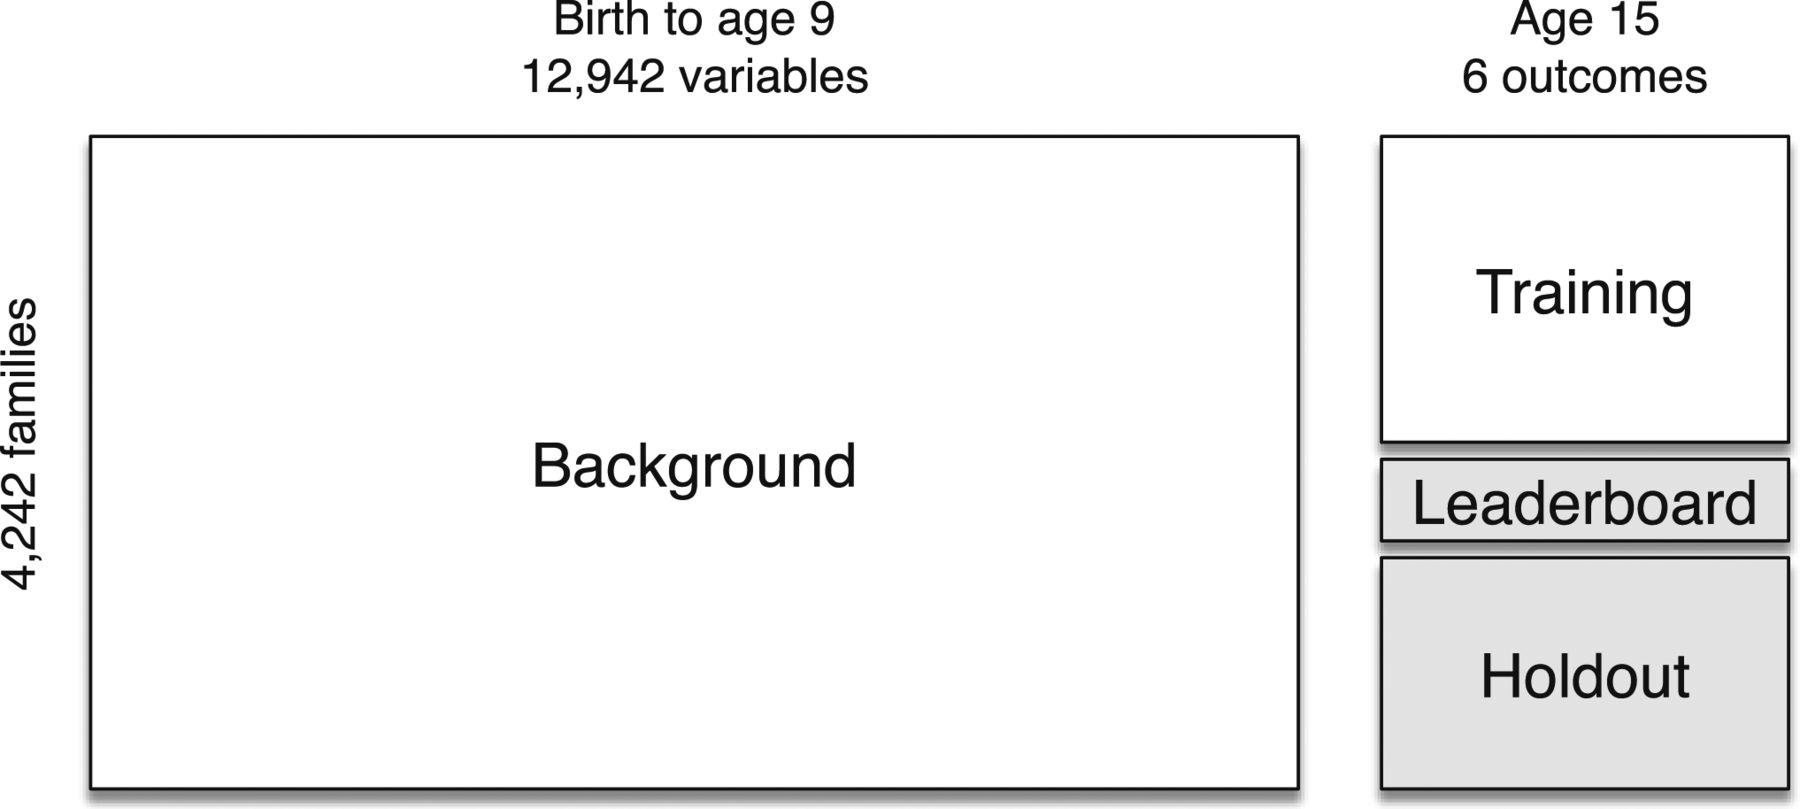
\includegraphics[width=\textwidth]{figures/salganik_measuring_2020_fig2}
\end{center}

\end{frame}
%%%%%%%%%%%%%%%%%%%%%%%%%
\begin{frame}

\begin{center}
\includegraphics[width=0.6\textwidth]{figures/ff_design_public_b9_15}
\end{center}

\end{frame}
%%%%%%%%%%%%%%%%%%%%%%%%%
\begin{frame}

\textbf{The Fragile Families and Child Wellbeing Study is a dataset of real people who have selflessly opened up their lives to us for the last 15 years so that their experiences can contribute to scientific research. By participating in the Fragile Families Challenge activity, you become a collaborator in this project. It is of the utmost importance that you respect the families in the data by using what they have told us responsibly.}

\end{frame}
%%%%%%%%%%%%%%%%%%%%%%%%%
\begin{frame}

\begin{itemize}
\item When you applied to get access to the data, you completed a data use agreement. Honor that agreement. \pause
\item After this activity you should delete the data from your computer. If you plan to do more research, you can download it again.
\end{itemize}

\end{frame}
%%%%%%%%%%%%%%%%%%%%%%%%
\begin{frame}

Many submissions to the Challenge had three main steps:
\begin{itemize}
\item data cleaning \pause
\item feature selection \pause
\item statistical learning \pause
\end{itemize}

\end{frame}
%%%%%%%%%%%%%%%%%%%%%%%%%
\begin{frame}

A reasonable goal for today is to upload a submission to the leaderboard

\end{frame}
%%%%%%%%%%%%%%%%%%%%%%%%%%
\begin{frame}

Questions about the activity?

\end{frame}
%%%%%%%%%%%%%%%%%%%%%%%%%%%%%%%
\begin{frame}

\begin{center}
\LARGE Good luck and enjoy
\end{center}

\end{frame}
%%%%%%%%%%%%%%%%%%%%%%%%%%%%%%%

\end{document}